\chapter{Teorie}
\label{2-Teorie}

\section{OpenStreetMap}
\label{OpenStreetMap}

\subsection{Vznik}
\label{vznik}
OpenStreetMap (OSM) je projekt, jež vznikl s cílem vytvoření a sběru 
volně dostupných geografických dat a následně jejich možné vizualizace
do topografických map. Projekt založil Steve Coast v červenci roku 
2004 v Anglii. Jako inspirace mu posloužil projekt Wikipedia.

Zprvu projekt využívalo jen pár nadšenců, postupem času ale získal
projekt popularitu. S nárůstem počtu uživatelů se zvyšoval i objem dat.
Bylo tedy nutné navýšit kapacitu a zabezpečení serverů.
Také bylo potřeba zlepšit síťové řešení a~infrastrukturu.
Tím je myšleno, že data byla rozdělena na více serverů.

V dubnu roku 2006 byla založena nadace OpenStreetMap Foundantion pro financování 
projektu jako takového (zaměstnanců, běhu, zajištění bezpečnosti serverů atd.). \cite{wikiOSM}

\subsection{Struktura dat}
\label{struktura dat}
OSM data jsou nyní uložena v objektově-relační databázi PostgreSQL. \cite{OSMserver}

Pro samotnou výměnu dat ale slouží souborový formát \textit{.osm}, který je postaven na značkovacím jazyku XML. 
Jeho výhodou je pevně daná struktura a snadná orientace v kódu pro člověka. 
Nevýhodou je ovšem větší objem dat, který lze ale snížit kompresí. 

Prvky (elementy) jsou v datovém modelu OSM rozděleny na:
\begin{itemize}
    \item uzel (node) 
    \item cesta (way)
        \subitem neuzavřená
        \subitem uzavřená
        \subitem plocha (area)
    \item relace (relation) 
\end{itemize}

\subsubsection{Uzel (node) }

Bodovým prvkem je v datovém modelu OSM tzv. uzel (node). Je definován jedinečným
identifikátorem ({\tt id}). 
Dále je ukládána verze uzlu, časový údaj, kdy byl do databáze přidán
a v jaké změně k tomu došlo ({\tt changeset}).
Každý uzel má svoje souřadnice definovány v souřadnicovém systému WGS~84 (EPGS 4326). 
Dále je možné připojit různé atributy (tzv. tagy) tj. klíče s hodnotou ({\tt tag~k=~v=}).
\\*
Příklad uzlu ve formátu \textit{osm}:

{\scriptsize \begin{lstlisting}
<node id="2905214905" visible="true" version="1" changeset="22804106" 
      timestamp="2014-06-08T06:57:20Z" user="Salamandr" 
      uid="1708065" lat="50.1036981" lon="14.3897278">
    <tag k="natural" v="tree"/>
    <tag k="source" v="bing:ortofoto"/>
</node>
\end{lstlisting} }

\subsubsection{Cesta (way) }

Označením pro liniový prvek je v datovém modelu OSM tzv. cesta (way). 
Každá cesta má svůj jedinečný identifikátor ({\tt id}) a základní atributy ({\tt visible, version, \ldots}), 
stejně jako je tomu u bodového prvku uzel.
Je vždy určena dvěma nebo více uzly, ze kterých se skládá. Uvedena je pouze reference na id uzlů, nikoliv jejich souřadnice.
Cestám lze taktéž přiřadit různé atributy.

Cesty se dále rozdělují na neuzavřené a uzavřené.
Uzavřené cesty mohou tvořit plošné objekty (area). Těmto plošným prvkům lze přiřadit speciální atributy jako je například les ({\tt landuse=forest}).

Příklad liniového prvku ve formátu \textit{osm}:

{\scriptsize
\begin{lstlisting}
<way id="87249754" visible="true" version="2" changeset="34489106"
     timestamp="2015-10-07T11:52:41Z" user="Petr Dlouhý" uid="17615">
    <nd ref="1014526199"/>
    <nd ref="1014525941"/>
    <nd ref="1014526337"/>
    <nd ref="1014526022"/>
    <nd ref="1014526277"/>
    <nd ref="1014525984"/>
    <tag k="highway" v="path"/>
    <tag k="source" v="bing:ortofoto"/>
</way>
\end{lstlisting}
}
      
\subsubsection{Relace (relation) }

Speciálním prvkem je relace (relation), do které lze zahrnout
jeden a více prvků. Mohou se do nich spojit prvky stejného druhu (uzel a uzel),
nebo různého (uzly, cesty nebo i relace).
Například dálnice je tvořena několika cestami (way), které
jsou zahrnuty do společné relace, např. \uv{Dálnice D1}. Nebo například turistická trasa
%%% ML: KCT jsem odstranil, nebo tato organizace data do OSM neposkytuje
může být relace sdružující jak liniové 
(cesty, pěšiny), tak i bodové (rozcestníky, vyhlídky, apod.) prvky.

%%% ML: nejde o wikipedii, ale wiki, vetu jsem zjednodusil (3x je, navic bez carrky)
Na wiki OpenStreetMap \cite{OSMfeatures} je uvedeno, které atributy jsou pro daný druhu prvku vhodné (dle komunity uživatelů OSM). Pokud je daný atribut použit nevhodně, tak mohou být související prvky v některých vykreslovačích chybně zobrazeny, viz kap. \ref{Vykreslovače}.
\begin{figure}[hbt]%[p]
    \centering
    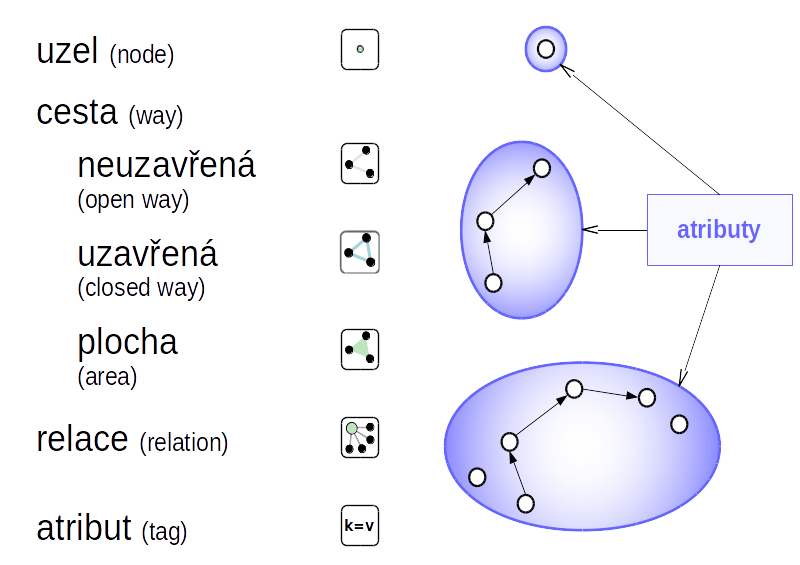
\includegraphics[scale=0.55]{./pictures/OSMelements.png}
    \caption{Rozdělení prvků OSM, vlastní tvorba (zdroj: vlastní)}
    \label{fig:rozdělení OSM prvků}
\end{figure}


\subsection{Změna licence}
\label{změna licence}

Původně byla data OSM a generované grafické dlaždice distribuovány pod licencí
Creative~Commons~AttributionShare~Alike 2.0 (CC~BY-SA~2.0).

Tato licence umožňovala užití (distribuci ale i editaci) díla (dat) pod podmínkou,
že bude uveden zdroj OpenStreetMap.org ve viditelné části
vytvořených mapových dlaždic \cite{OSMlicence}.

  \begin{figure}[hbt]
    \centering
      
\includegraphics[scale=0.75]{./pictures/attribution_example.png}
      \caption{Příklad umístění licence 
                (zdroj: \url{http://www.openstreetmap.org/copyright})}
      \label{fig:attribution_example}
  \end{figure} 

V roce 2012 byla licence publikovaných dat změněna na Open Data Commons
Open Database Licence (ODbL).
Důvodem byla lepší licenční ochrana dat v databázi. 
Původní licence (CC BY-SA) chránila data pouze pomocí autorského zákona. 
Obě licence jsou sice postaveny na principu \uv{Uveďte autora} a \uv{Zachovejte licenci}. Rozdíl mezi nimi je ten, že pokud někdo pod licencí CC BY-SA vytvoří mapu (nebo jiné dílo), musí zachovat stejnou licenci.
Nemusí však uvolnit přímo data, která pro tvorbu mapy použil.

%%% ML: tento odstavec vyzaduje revizi
Data OSM pod novou (ODbL) licencí, je možné jakkoli upravit,
%%% ML: ta licence muze byt opravdu jina, mel jsem pocit, ze to musi
%%% byt opet ODbL?
a zveřejnit pod jakoukoli jinou licencí, 
která je kompatibilní s ODbL a 
za podmínky, že dojde k uvolnění souvisejících doplňků a vylepšení. \cite{OSMlicenceChange}.

Změna licence přinesla problém
s~daty, které byly poskytnuty projektu za podmínek předchozí licence
(CC~BY-SA~2.0). Bylo nutné se dotázat každého z~dřívějších
přispěvatelů dat, ať už právnických osob, tak i fyzických osob,
zdali souhlasí s tím, aby jejich data byla distribuována pod novou licencí (ODbL).
U~přispěvatelů, kteří k tomuto nesvolili nebo se nevyjádřili,
bylo nutné jejich příspěvky z~databáze OSM vymazat.
Tato situace nastala pouze ve zlomku případů (méně než 1 \%).
Nejvíce tato změna licencí ohrozila data v zemích jako je Polsko a Nový Zéland. \cite {OSMlicenceIssue}

V současnosti jsou tedy data OSM distribuována pod licencí ODbL a
generované grafické dlaždice pod licencí CC BY-SA 4.0. \cite{OSMlicence}

\subsection{Licence ODbL}
Licence ODbL
se zabývá právní ochranou databází, včetně
veškerých autorských a příbuzných práv k databázi.

Licence ODbL umožňuje:
\begin{itemize}
    \item    kopírovat, distribuovat a užívat data
    \item    vytvářet nová data z původních
    \item    měnit původní data
\end{itemize}

Při použití databáze s licencí ODbL, je
nutné připojit kopii přesného znění této licence.
Při nakládnání s databází ponechat nedotčena veškerá autorská práva a
uvést jejich zdroj (nebo autora).
Veškeré odvozené databáze musí splňovat podmínky ODbl,
tj. buď přímo licence ODbL nebo licence s ní kompatibilní. \cite{ODbL}


\subsection{Zdroje dat}
\label{Zdroje dat}
Snahou je, aby mapová data tvořili jedinci prvotním
sběrem dat, tj. měřením vlastními GNSS (GPS, Glonass) přijímači a
znalostí místních poměrů (uzavřené silnice, stezky atd.).  Takto
vzniklé dílo volně užívat k vlastním potřebám. Komunita přispěvatelů se
zprvu pomalu, později poměrně rychle rozrostla a dnes čítá 3,7 milionů
registrovaných uživatelů s alespoň jednou vytvořenou změnou v~OSM. Z toho je 2,7 milionů účtů aktivních přispěvatelů.\cite{OSMstats}

Takto vzniklé mapové podklady byly vhodné i pro další projekt, dnes již
velice rozšířený a známý jako GeoCashing (GC). Projekt GC začal užívat mapové
podklady OSM a zároveň jeho uživatelé začali sami přispívat do OSM. 

Přispěvatelé dat do OSM musí respektovat licenci projektu ODbL.
%%% ML: nebo s ni kompatibilni?
Tudíž i jejich zdroj dat musí splňovat podmínky této licence.
Proto by měli
všechny svoje změny, které v OSM vytvoří, řádně ozdrojovat atributem
s~klíčem 
{\tt source}.
V případě vlastního sběru dat se vyplňuje hodnotou
{\tt source=survey},
popřípadě uvést zdroj, odkud čerpali. Pokud tuto povinnost poruší a
použijí zdroj, jež není kompatibilní s licenční politikou OSM, tak ostatní 
přispěvatelé do~OSM tuto změnu, aby předešeli sporům, odstraní. 
V tomto případě dojde k odstranění celé sady změn, byť by v~ní byl pouze jeden prvek, jenž licenční podmínky poruší.

Druhým významným zdrojem dat jsou soukromé subjekty (společnosti).
Většinou jde o podkladové zdroje dat, například ortofoto, které jsou
vhodné pro obkreslování silničních sítí z~leteckých nebo
satelitních snímků a pod.
%%% ML: navrhuji tuto vetu preskocit
% V~jejich případě to bylo řešeno písemným svolením, nebo smlouvou.
Významným zdrojem těchto dat jsou mapy vyhledávače Bing od společnosti
Microsoft. Ta svolila použít jejich letecké snímky většiny
obydlené pevniny \footnote{\url{http://wiki.openstreetmap.org/wiki/Bing}}.

Třetím zdrojem dat a zároveň postupně dominujícím, co do jeho obsahu, jsou
datové sady ze státního sektoru. Tyto datové sady jsou vzhledem ke své kvalitě a konzistenci velmi žádoucím zdrojem
dat pro OSM.

\subsection{Importy}
\label{Importy}
%%% ML: neobratne receno, ale muzeme nechat
Výraz import v tomto případě znamená začlenění většího množství dat z datové sady nebo datových sad
z~jednoho datového úložiště do jiného uložiště (např. databázových serverů). Při velkých objemech dat
%%% ML: o bezchybnosti bych nemluvil, zkusil jsem alespon minimalne preformulovat
se využívá automatizace pomocí skriptů nebo programů, které samotný proces importu provednou.

Datové importy z veřejných databází do databáze OSM jsou velmi cenné. 
Otevřené geografické, ale i jiné, datové zdroje státních či veřejných institucí 
financovaných státem jsou často komplexní. Obsahují celistvý
soubor dat, který daná instituce vyžaduje ke svému chodu. Jistá nevýhoda tu 
ale může být, data nemusí být vždy úplně aktuální. Některá data mohou 
být totiž zveřejněna i s větším časovým odstupem.

V rámci České republiky proběhlo již několik hromadných datových importů do OSM. Jak 
již bylo řečeno, časově nejnáročnější je samotná příprava importu.
V~případě importu dat do OSM, nejen napsání skriptu, ale i nutná diskuze tohoto záměru
na~diskuzní konferenci Talk-cz. 

\subsection{Talk-cz}
\label{Talk-cz}
%%% ML: prilis polopatisticke, ale nechte to tak
Tato diskuze probíhá posíláním emailových zpráv do společné konference (diskuzního fóra). 
Uživatelům chodí emaily z probíhající diskuze. Pokud na nějaký
chtějí reagovat, tak pošlou zprávu na emailovou adresu konference. Musí ale do předmětu zprávy (emailu) napsat Re: a předmět zprávy, na kterou reagují.
Server tyto zprávy řadí pomocí 
předmětu a času. Diskuze je poté k dispozici na webových stránkách.\footnote{\url{http://lists.openstreetmap.org/listinfo/talk-cz}}

\subsection{Vykreslovače}
\label{Vykreslovače}
Na hlavní stránce OSM (\url{http://www.openstreetmap.org}) je k dispozici mapová aplikace. Ta nabízí pět
„základních“ přednastavených vrstev vykreslených z~dat OSM.
%%%: SRS nijak neusnadnuje vykreslovani, slovo jsem vynechal
Pro vykreslení dat do grafických dlaždic se používá takzvané pseudo Mercatorovo
zobrazení nebo Web Mercator (EPSG 3857). Toto zobrazení je vhodné pro celý povrch Země (až na velké zkreslení u pólů). 
První, kdo zobrazení Web Mercartor použil, byla společnost Google pro svoje mapy Google Maps.\cite{WebMercator}
%%% ML: mozna dodat screenshoty do prilohy?

\begin{itemize}
  \item Standardní vrstva - vykresluje všechny prvky kartograficky \uv{přiměřeně}.
  \item Cyklomapa - zdůrazňuje cyklostezky, výškopis. 
  \item Dopravní mapa - zdůrazňuje silniční a železniční sítě.
  \item MapQuest Open - podkladová mapa pro potřeby GeoCaching.
  \item Humanitární mapa - zdůrazňuje důležité veřejné služby a potlačuje ostatní prvky. 
\end{itemize}

Existují další projekty, jež kombinují data OSM a jiných zdrojů, s cílem tvorby tematických map.
Například mapu turistických a cyklistických tras vykresluje
pro celou Evropu projekt \textit{mtbmap}.\footnote{mtbmap.cz}

%%% priklad? mozna dodat hezky screenshot?
Dalšími zajímavými projekty jsou například ty, které k 2D polohopisných datům přidávají „třetí“ rozměr a
vytvářejí tzv. 2.5D mapu. Většinou jde o 3D zobrazení budov, mostů (dle
atributů), popřípadě i stromů.

%%% http://demo.f4map.com/#lat=50.1036063&lon=14.3898880&zoom=19


\section{Otevřená data}
\label{opendata}

%%% ML: chybi mi tu reference pro tuto kapitolu, ze ktere jste cerpal (stupne otevrenosti)
Myšlenka otevřených dat (open data) vznikla v USA.
Pokud vzniknou jakákoli data z veřejných peněz, měla by tedy být
veřejně přístupná. Některé studie uvádí, že tento jev měl kladný efekt na tamní ekonomiku.
%%% ML: navrhuji presnout do seznamu literatury, uz tak mate dost poznamek pod carou
\footnote{\url{http://www.worldbank.org/content/dam/Worldbank/document/Open-Data-for-Economic-Growth.pdf}}
\footnote{\url{http://www.otevrenadata.cz/res/data/001/003498.pdf}}

Proto jako první hlavní zdroj pro OSM byly satelitní snímky povrchu Země (Landsat) %\footnote{\url{http://landsat.usgs.gov/}}
a digitální model terénu (projekt SRTM) %\footnote{\url{http://www2.jpl.nasa.gov/srtm/}}
s~rozlišením 30x30 m od NASA (pro pozdější vykreslení vrstevnic).

Trend otevírání dat se začal rozšiřovat zprvu do zemí západní Evropy
(Velké Británie, Francie či Německa), ale i země mimo Evropu.\cite{OpendataTrends}

V České republice se tomuto tématu věnuje Fond Otakara Motejla. Jedním z jeho hlavních projektů jsou právě Otevřená data. Fond spolupracuje s nadací Society Fund
Praha a Rekonstrukce Státu.
V rámci těchto uskupení je vyvíjen tlak na transparentnost veřejné správy,
zveřejňování smluv a dat státních institucí, jelikož jejich získání a údržba byla
placena z~veřejných zdrojů.

\newpage
Otevřená data lze dělit na 5 stupňů,
dle otevřenosti.

\begin{figure}[hbt]%[p]
    \centering
    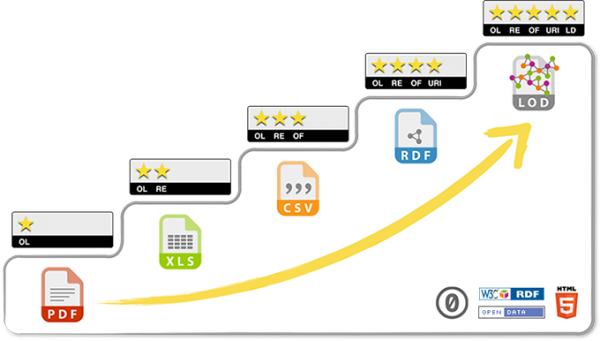
\includegraphics[width=0.8\textwidth]{./pictures/5star-steps.png}
    \caption{Stupně otevřenosti dat, převzato z \url{http://5stardata.info}}
    \label{fig:Stupně otevřenosti dat}
\end{figure}

\begin{itemize}

    \item   Data jsou dostupná v WWW stránek s jasnými licenčními
            podmínkami. Není zde žádný požadavek na datový formát,
            a proto není brán jako dostatečný způsob zveřejňování dat.
            Těmito daty ku příkladu jsou Webové Mapové Služby (WMS).
            Jsou veřejně k dispozici, avšak nezveřejňují přímo data,
            ale jen obrázky z nich generované.

    \item   Zveřejněná data jsou již ve strojově čitelném formátu,
            který je veřejně dobře znám. Nejčastěji se jedná
            o~charakter tabulky. Musí umožňovat přístup k~jednotlivým
            řádkům a obsahu buněk.

    \item   Třetí stupeň navíc od druhého vyžaduje, aby k~jeho čtení
            nebyl vyžadován speciální (uzavřený) software. Spadají sem tedy dokumenty formátů
            OpenOffice (Office Open XML, OpenDocument).
        \\* Pro~prostorová data například formáty GML, KML nebo
            GeoPackage.

    \item   U stupně otevřenosti 4 je v distribuované datové sadě
            povinnost zavést identifikaci entity ve tvaru
            Internationalized Resource Identifier (IRI).

    \item   U nejvyššího možného stupně otevřenosti je vyžadováno, aby
            distribuce splňovala standardy propojených dat (Linked
            Data). \cite{OpendataStupne}

\end{itemize}
%% http://opendata.gov.cz/standardy:stupne-otevrenosti

Díky této iniciativě došlo v rámci České republiky ke zveřejnění
dat státních úřadů s různým úspěchem a stupněm otevřenosti.
Avšak tento trend zpřístupnění a zveřejňování pozvolna pokračuje.
Příkladem je Ministerstvo vnitra, Ministerstvo financí nebo Český úřad zeměměřický a katastrální (RÚIAN).


\section{IPR Praha}
\label{IPR Praha}
IPR Praha je zkratka názvu pro Institut plánování a rozvoje
hlavního města Prahy. Tento institut se věnuje urbanismu, architektuře
a rozvoje města Prahy. Hlavním úkolem IPR je tvorba územního plánu
hlavního města Prahy. Významným úkolem IPR je zajišťovat zpracování geografických
informací. Od roku 2002 poskytuje
na~svých stránkách zdarma webové aplikace bez limitu využití.
V rámci tzv. Pražského geoportálu došlo k jejich většímu využívání.
Na~základě platných Pravidel pro poskytování dat a výstupů z~datových
souborů a datového skladu Geografického byly ode dne 1.~4.~2015
zveřejněny datové soubory a další webové služby poskytované IPR. Data byla
%%% ML: snazil jsem se v cele praci sjednotit zapis na CC BY-SA (mate to ruzne snad ve vsech moznych variantach)
uveřejněna pod licencí CC BY-SA 4.0. \cite{IPR}

\subsection{Licence CC BY-SA 4.0}
\label{licence CC BY-SA 4.0}
Licence Creative Commons Attribution-ShareAlike 4.0 International (CC BY-SA 4.0)
je zde uvedena ve zjednodušeném znění.

Uživatel smí:

\begin{itemize}
    \item   sdílet - rozmnožovat a distribuovat materiál prostřednictvím jakéhokoli média v jakémkoli formátu
    \item   upravovat - remixovat, změnit a vyjít z původního díla
\end{itemize}
a to pro jakýkoliv účel, i komerční.

Poskytovatel licence nemůže odvolat tato oprávnění do té doby, dokud dodržujete licenční podmínky.

Uveďte původ — Je Vaší povinností uvést autorství, poskytnout s dílem odkaz
na~licenci a vyznačit Vámi provedené změny. Toho můžete docílit jakýmkoli
rozumným způsobem, nicméně nikdy ne způsobem naznačujícím, že by poskytovatel
licence schvaloval nebo podporoval Vás nebo Váš způsob užití díla.

Zachovejte licenci — Pokud budete toto dílo upravovat, pozměňovat nebo
na~něj navazovat, musíte svoje odvozená díla vystavovat pod stejnou
licencí jako původní dílo.\cite{CCBYSA4}
